\documentclass[hyperref=unicode]{beamer}

\usepackage[absolute,overlay]{textpos}
\usepackage{graphicx}
\usepackage{adjustbox}
\usepackage{chemfig}
\usepackage[version=4]{mhchem}
\usepackage{wrapfig}
\usepackage{multirow}
\adjustboxset*{center}
\usepackage{caption}
\usepackage{chemformula}
\usepackage{elements}

%dělení slov
\usepackage{ragged2e}
\let\raggedright=\RaggedRight
%konec dělení slov

\usepackage{fontspec}
\usepackage{unicode-math}

\usepackage{polyglossia}
\setdefaultlanguage{czech}

\def\uv#1{„#1“}

\mode<presentation>{\usetheme{Madrid}}
\DefineNamedColor{named}{pozadi}{RGB}{200,200,200}
\usecolortheme{crane}

\setbeamertemplate{footline}[frame number]

\addtobeamertemplate{frametitle}{
	\let\insertframetitle\insertsectionhead}{}
\addtobeamertemplate{frametitle}{
	\let\insertframesubtitle\insertsubsectionhead}{}

\makeatletter
\CheckCommand*\beamer@checkframetitle{\@ifnextchar\bgroup\beamer@inlineframetitle{}}
\renewcommand*\beamer@checkframetitle{\global\let\beamer@frametitle\relax\@ifnextchar\bgroup\beamer@inlineframetitle{}}
\makeatother
\setbeamercolor{section in toc}{fg=blue}
\setbeamertemplate{section in toc shaded}[default][100]

\title[Crisis] % (optional, only for long titles)
{Ramanova spektroskopie}

\author % (optional, for multiple authors)
{Zdeněk Moravec, C12/316, hugo@chemi.muni.cz}

\date{} %hide date on titlepage

\subtitle{C5060 Metody chemické výzkumu}

\begin{document}
\frame{\titlepage}

\section{Osnova}
\frame{
	\frametitle{}
	\vfill
	\begin{itemize}
	\item Základní principy Ramanovy spektroskopie
	\begin{itemize}
		\item Ramanův rozptyl
		\item Polarizovatelnost
	\end{itemize}
	\item Ramanovy spektrometry a mikroskopy
	\item Využití Ramanovy spektroskopie v praxi
	\item Aplikace
	\begin{itemize}
		\item Chemie
		\item Restaurování uměleckých předmětů
		\item Biologie
	\end{itemize}
	\item Informace o přístrojovém vybavení UCH
	\end{itemize}
	\vfill
}

\section{Ramanův rozptyl}
\frame{
	\frametitle{}
	\vfill
	\begin{itemize}
	\item Při interakci elektromagnetického záření s hmotou může dojít k absorbci, přenosu a rozptylu.
	\item Rozptyl může být pružný a nepružný.
	\item Při pružném rozptylu nedochází k výměně energie mezi zářením a hmotou. Tento byl popsán britským fyzikem Lordem Rayleighem, po němž je pojmenován.\footnote[frame]{\url{http://hyperphysics.phy-astr.gsu.edu/hbase/atmos/blusky.htm\#c2}}
	\item Při nepružném rozptylu naopak k výměně energie mezi zářením a hmotou dochází. Tento jev byl popsán v roce 1928 Sirem Chandrasekhara Venkata Ramanem.\footnote[frame]{\href{https://vesmir.cz/cz/casopis/archiv-casopisu/2024/cislo-4/objev-z-lodni-paluby.html}{Objev z lodní paluby}} Pojmenován byl po objeviteli \em{Ramanův efekt} nebo \em{Smekalův-Ramanův efekt}. Za tento objev obdržel sir Raman Nobelovu cenu za fyziku v roce 1930.\footnote[frame]{\url{http://www.nobelprize.org/nobel_prizes/physics/laureates/1930/raman-lecture.pdf}}
\end{itemize}
	\vfill
}

\frame{
	\frametitle{}
	\vfill
	\begin{columns}
		\begin{column}{0.5\textwidth}
			\begin{figure}
				\adjincludegraphics[height=.6\textheight]{../img/Sir_CV_Raman.jpg}
				\caption*{Sir Raman.\footnote[frame]{Zdroj: \href{https://commons.wikimedia.org/wiki/File:Sir_CV_Raman.JPG}{Nobel Foundation/Commons}}}
			\end{figure}
		\end{column}
		
		\begin{column}{0.5\textwidth}
			\begin{figure}
				\adjincludegraphics[width=\textwidth]{../img/Raman_1928_Benzene_Spectrum.png}
				\caption*{Ramanovo spektrum benzenu z roku 1928.\footnote[frame]{Zdroj: \href{https://commons.wikimedia.org/wiki/File:1928_Benzene_Raman_Spectrum.png}{C. V. Raman/Commons}}}
			\end{figure}
		\end{column}
	\end{columns}
	\vfill
}

\frame{
	\frametitle{}
	\vfill
	\begin{itemize}
	\item Ramanův efekt může být popsán jako nepružná srážka fotonu s molekulou, jejímž výsledkem je změna vibračního nebo rotačního stavu molekuly.\footnote[frame]{\href{http://www.4oci.cz/rozptyl-svetla-nejvsednejsi-jev-v-prirode-nebo-div-moderni-optiky_4c290}{Malíšek V.: "Rozptyl světla - nejvšednější jev v přírodě, nebo div moderní optiky?", str. 62-64}}
	\item \emph{Stokesův rozptyl}: vzorek přijme část energie od záření a emituje foton s nižší energií.
	\item \emph{anti-Stokesův rozptyl}: vzorek ztratí část energie a emituje foton s vyšší energií.
	\item Stokesovy linie jsou intenzivnější než anti-Stokesovy. Poměr intenzit je teplotně závislý, čehož lze využít pro měření teploty.
	\begin{itemize}
	\item \scalebox{1.5}{$\frac{I_{as}}{I_s} = \frac{(\nu_i + \nu)^4}{(\nu_i - \nu)^4}\ e^{-\frac{h\nu_i}{kT}}$}
	\end{itemize}
	\item Hodnota Ramanova posunu je \emph{nezávislá} na energii (vlnové délce) použitého laseru.
	\end{itemize}
	\vfill
}

\frame{
	\frametitle{}

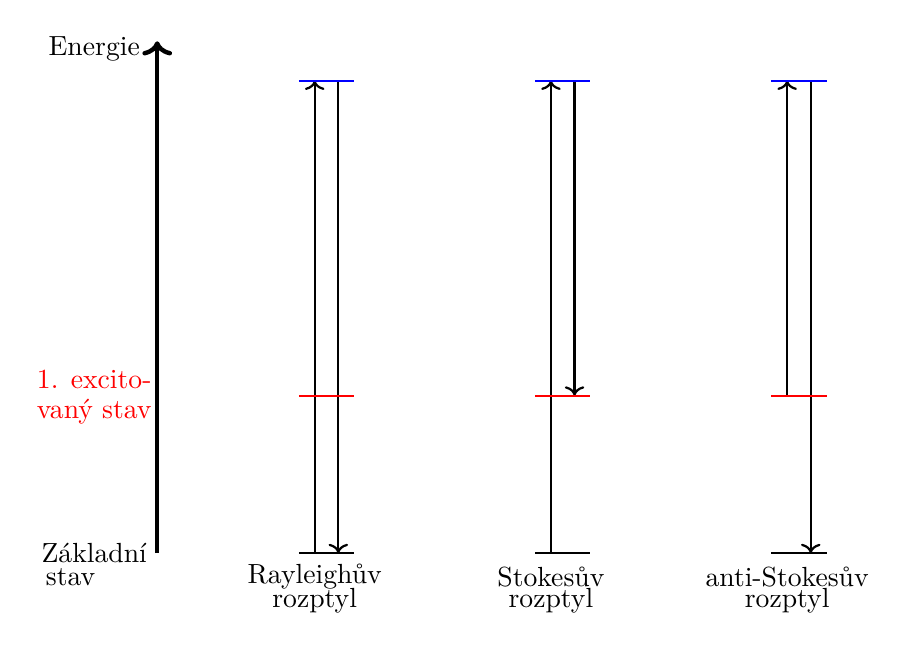
\begin{tikzpicture}
\node at (-0.8,6.4) {Energie};
\draw [ultra thick,->] (0,0) -- (0,6.5);
\node at (-0.8,0) {Základní};
\node at (-1.1,-0.3) {stav};
\node [red] at (-0.8,2.2) {1. excito-};
\node [red] at (-0.8,1.8) {vaný stav};

\draw [thick,->] (2,0) -- (2,6);
\draw [thick,<-] (2.3,0) -- (2.3,6);
\draw[thick] (1.8,0) -- (2.5,0);
\draw[thick,red] (1.8,2) -- (2.5,2);
\draw[thick,blue] (1.8,6) -- (2.5,6);
\node at (2,-0.3) {Rayleighův};
\node at (2,-0.6) {rozptyl};

\draw [thick,->] (5,0) -- (5,6);
\draw [thick,<-] (5.3,2) -- (5.3,6);
\draw[thick] (4.8,0) -- (5.5,0);
\draw[thick,red] (4.8,2) -- (5.5,2);
\draw[thick,blue] (4.8,6) -- (5.5,6);
\node at (5,-0.3) {Stokesův};
\node at (5,-0.6) {rozptyl};

\draw [thick,->] (8,2) -- (8,6);
\draw [thick,<-] (8.3,0) -- (8.3,6);
\draw[thick] (7.8,0) -- (8.5,0);
\draw[thick,red] (7.8,2) -- (8.5,2);
\draw[thick,blue] (7.8,6) -- (8.5,6);
\node at (8,-0.3) {anti-Stokesův};
\node at (8,-0.6) {rozptyl};
\end{tikzpicture}
}

\section{Polarizovatelnost}
\frame{
	\frametitle{}
	\vfill
	\begin{itemize}
	\item Polarizovatelnost ($\alpha$) popisuje deformovatelnost elektronové hustoty v okolí molekuly působením elektromagnetického záření, nebo přesněji elektrického pole generovaného fotonem.\footnote[frame]{\url{https://en.wikipedia.org/wiki/Polarizability}}$^,$\footnote[frame]{\url{http://chemwiki.ucdavis.edu/Physical_Chemistry/Physical_Properties_of_Matter/Intermolecular_Forces/Polarizability}}
	\item Je to \emph{tensor druhého řádu}, tzn. že ji lze popsat maticí $3\times3$.\footnote[frame]{\url{https://en.wikipedia.org/wiki/Tensor}}
	\end{itemize}
	\begin{columns}
	\begin{column}{0.5\textwidth}
		\begin{figure}
			\adjincludegraphics[height=.3\textheight]{../img/tensor-comp.png}
			\caption*{Složky tensoru polarizovatelnosti.\footnote[frame]{Zdroj: \href{https://commons.wikimedia.org/wiki/File:Components_stress_tensor.svg}{Sanpaz/Commons}}}
		\end{figure}
	\end{column}
	\begin{column}{0.5\textwidth}
\scalebox{1}{$\alpha =
\begin{bmatrix}
\alpha_{xx} & \alpha_{xy} & \alpha_{xz}\\
\alpha_{yx} & \alpha_{yy} & \alpha_{yz}\\
\alpha_{zx} & \alpha_{zy} & \alpha_{zz}\\
\end{bmatrix}$}
	\end{column}
	\end{columns}
	\vfill
}

\frame{
	\frametitle{}
	\vfill
		\begin{itemize}
			\item Polarizovatelnost ($\alpha$) je ovlivněna několika faktory:
			\begin{itemize}
				\item Čím více elektronů má atom, tím slaběji je k sobě váže a tím je polarizovatelnost větší.
				\item Čím je elektron více vzdálen od kladného jádra, tím je pohyblivější a zvyšuje polarizovatelnost atomu.
				\item Orientací molekuly vůči vnějšímu elektrickému poli.
			\end{itemize}
			\item Ramanův rozptyl lze popsat rovnicí pro indukovaný dipólový moment:
			\item $\vec{p} = \alpha \vec{E} \cos(2 \pi \nu_0t) + \frac{1}{2} \frac{\delta\alpha}{\delta q}q\vec{E}\{\cos[2\pi(\nu_0-\nu_{vib})t] + \cos[2\pi(\nu_0+\nu_{vib})t]\}$
			\item První člen odpovídá Rayleighovu rozptylu, druhý a třetí pak Ramanovu (Stokes a anti-Stokes).
		\end{itemize}
	\vfill
}

\section{Ramanova spektroskopie}
\frame{
	\frametitle{}
	\vfill
	\begin{itemize}
	\item Ramanova spektroskopie je komplementární metodou k infračervené spektroskopii.
	\item Citlivost je nižší než v případě IR spektroskopie.
	\item Je vhodnější pro nepolární vazby a umožňuje pozorovat vibrace i na nižších vlnočtech než MIR spektroskopie ($<$400 cm$^{-1}$).
	\item Umožňuje snadné měření vodných roztoků (voda poskytuje slabý signál).
	\item Aby byla vibrace aktivní v IR spektroskopii, musí během ní docházet ke změně vektoru dipólmomentu molekuly.
	\item Aby byla vibrace aktivní v Ramanově spektroskopii, musí během ní docházet ke změně \emph{tensoru polarizovatelnosti} molekuly (viz rovnice na předchozím slidu).
	\item Pokud má molekula \emph{střed symetrie}, mohou být vibrace aktivní buď v IR nebo v RA, ale ne v obou zároveň.
	\end{itemize}
	\vfill
}

\frame{
	\frametitle{}

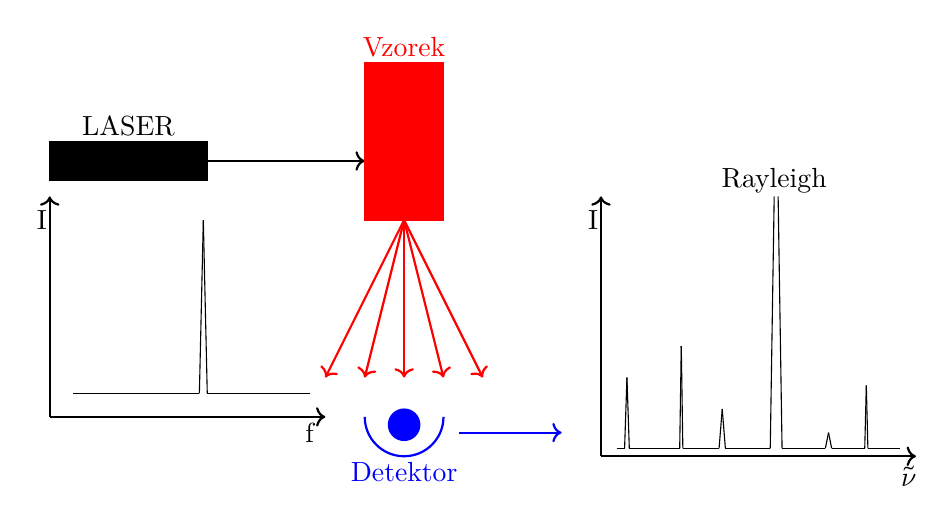
\begin{tikzpicture}
\node at (9,10.2) {LASER};
\draw [fill=black] (10,10) rectangle (8,9.5);
\draw [thick,->] (10,9.75) -- (12,9.75);

\draw [thick,<-] (8,9.3) -- (8,6.5);
\node at (7.9,9) {I};
\draw [thick,->] (8,6.5) -- (11.5,6.5);
\node at (11.3,6.3) {f};
\draw (8.3,6.8) -- (9.9,6.8);
\draw (10,6.8) -- (11.3,6.8);
\draw (9.9,6.8) -- (9.95,9);
\draw (10,6.8) -- (9.95,9);


\draw [fill=red,red] (12,11) rectangle (13,9);
\node [red] at (12.5,11.2) {Vzorek};
\draw [thick,->,red] (12.5,9) -- (12.5,7);
\draw [thick,->,red] (12.5,9) -- (13.5,7);
\draw [thick,->,red] (12.5,9) -- (11.5,7);
\draw [thick,->,red] (12.5,9) -- (13.0,7);
\draw [thick,->,red] (12.5,9) -- (12,7);

\draw [thick,blue] (12.0,6.5) arc [radius=0.5, start angle=180, end angle=360];
\draw [blue,fill=blue] (12.5,6.4) circle [radius=0.2];
\draw [thick,->,blue] (13.2,6.3) -- (14.5,6.3);
\node [blue] at (12.5,5.8) {Detektor};

\draw [thick,<-] (15.0,9.3) -- (15.0,6.0);
\node at (14.9,9.0) {I};
\draw [thick,->] (15.0,6.0) -- (19,6.0);
\node at (18.9,5.75) {$\tilde\nu$};

\draw (17.15,6.1) -- (17.2,9.3);
\draw (17.3,6.1) -- (17.25,9.3);

\draw (16.5,6.1) -- (16.54,6.6);
\draw (16.58,6.1) -- (16.54,6.6);

\draw (16.0,6.1) -- (16.02,7.4);
\draw (16.04,6.1) -- (16.02,7.4);

\draw (15.3,6.1) -- (15.33,7.0);
\draw (15.36,6.1) -- (15.33,7.0);

\draw (17.85,6.1) -- (17.89,6.3);
\draw (17.93,6.1) -- (17.89,6.3);

\draw (18.35,6.1) -- (18.37,6.9);
\draw (18.39,6.1) -- (18.37,6.9);

\draw (15.2,6.1) -- (15.3,6.1);
\draw (15.36,6.1) -- (16.0,6.1);
\draw (16.04,6.1) -- (16.5,6.1);
\draw (16.58,6.1) -- (17.15,6.1);
\draw (17.3,6.1) -- (17.85,6.1);
\draw (17.93,6.1) -- (18.35,6.1);
\draw (18.39,6.1) -- (18.8,6.1);

\node at (17.2,9.5) {Rayleigh};

\end{tikzpicture}
}

\section{Spektrometry}
\frame{
	\frametitle{}
	\vfill
	\begin{itemize}
	\item Podle optické soustavy
	\begin{itemize}
	\item Disperzní
	\item FT-Raman
	\item Mikroskopy
	\end{itemize}
	\item Podle vlnové délky laseru
	\begin{itemize}
	\item UV
	\item VIS
	\item NIR
	\end{itemize}
	\end{itemize}
	\vfill
}

\subsection{Disperzní spektrometry}
\frame{
	\frametitle{}
	\vfill
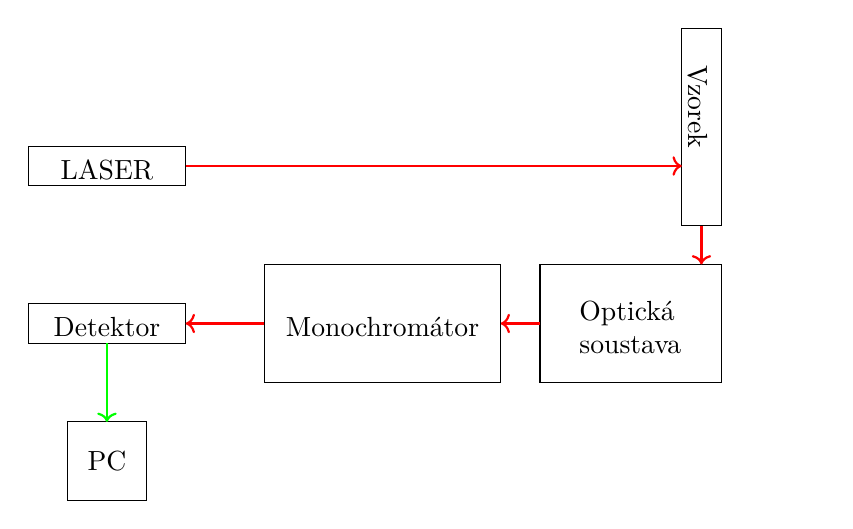
\begin{tikzpicture}
\draw [fill=white] (2,10) rectangle (0,9.5);
\node at (1,9.7) {LASER};

\draw [fill=white] (0,7.5) rectangle (2,8);
\node at (1,7.7) {Detektor};

\draw [fill=white] (0.5,5.5) rectangle (1.5,6.5);
\node at (1,6) {PC};

\draw [fill=white] (6.5,7) rectangle (8.8,8.5);
\node at (8.5,7.7) [text width = 3cm] {Optická \\ soustava};

\draw [thick,->, red] (8.55,9.0) -- (8.55,8.5);
\draw [thick,->, red] (6.5,7.75) -- (6,7.75);

\draw [fill=white] (3,7) rectangle (6,8.5);
\node at (4.5,7.7) {Monochromátor};

\draw [fill=white] (8.3,11.5) rectangle (8.8,9.0);
\node at (8.5,10.5) [rotate=270] {Vzorek};

\draw [thick,->, red] (2,9.75) -- (8.3,9.75);

\draw [thick,->, red] (3,7.75) -- (2,7.75);

\draw [thick,->, green] (1,7.5) -- (1,6.5);

\end{tikzpicture}
	\vfill
}

\subsection{FT-RA spektrometry}
\frame{
	\frametitle{}
	\vfill
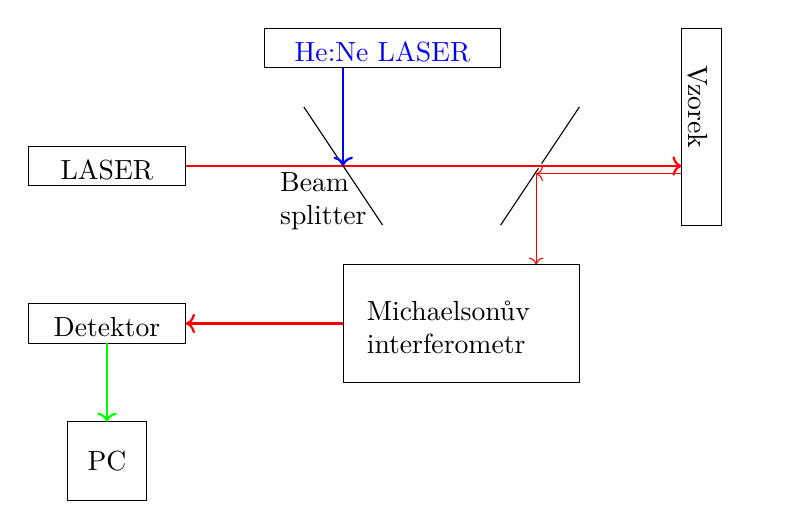
\begin{tikzpicture}
\draw [fill=white] (2,10) rectangle (0,9.5);
\node at (1,9.7) {LASER};

\draw [fill=white] (3,11) rectangle (6,11.5);
\node[blue] at (4.5,11.2) {He:Ne LASER};

\draw [fill=white] (0,7.5) rectangle (2,8);
\node at (1,7.7) {Detektor};

\draw [fill=white] (0.5,5.5) rectangle (1.5,6.5);
\node at (1,6) {PC};

\draw [fill=white] (4,7) rectangle (7,8.5);
\node at (6.8,7.7) [text width=5cm] {Michaelsonův \\ interferometr};

\node at (4.7,9.3) [text width=3cm] {Beam \\ splitter};

\draw [fill=white] (8.3,11.5) rectangle (8.8,9.0);
\node at (8.5,10.5) [rotate=270] {Vzorek};

\draw [thick,->, red] (2,9.75) -- (8.3,9.75);
\draw [thin] (3.5,10.5) -- (4.5,9.0);
\draw [thick,->, blue] (4,11) -- (4,9.75);

\draw [thin] (7.0,10.5) -- (6.52,9.78);
\draw [thin] (6.48,9.72) -- (6.0,9.0);

\draw [thin,->, red] (8.3,9.65) -- (6.45,9.65);
\draw [thin,->, red] (6.45,9.65) -- (6.45,8.5);

\draw [thick,->, red] (4,7.75) -- (2,7.75);

\draw [thick,->, green] (1,7.5) -- (1,6.5);

\end{tikzpicture}
	\vfill
}

\frame{
	\frametitle{}
	\vfill
	\adjincludegraphics[width=115mm]{../img/FRA106FT-RA.png}
	\vfill
}

\subsection{LASER}
\frame{
	\frametitle{}
	\vfill
	\begin{itemize}
	\item \textbf{L}ight  \textbf{A}mplification by  \textbf{S}timulated  \textbf{E}mission of  \textbf{R}adiation.
	\item Zesilování světla stimulovanou emisí záření.\footnote[frame]{VRBOVÁ, Miroslava. \emph{Lasery a moderní optika.} Praha : Prometheus, 1994. 474 s. ISBN 80-85849-56-9.}
	\item První laser byl sestrojen roku 1957, teoreticky byl předpovězen (resp. stimulovaná emise) již roku 1917 Albertem Einsteinem.\footnote[frame]{\href{http://qoqi.physik.uni-erlangen.de/teaching/SS2012/Daten/Einstein.pdf}{Zur Quantentheorie der Strahlung}}
	\item Jde o koherentní a monochromatický zdroj záření.\footnote[frame]{\href{https://www.youtube.com/watch?v=R_QOWbkc7UI}{Laser principle animation}}
	\begin{itemize}
	\item Koherentní - na dlouhém úseku mezi jednotlivými vlnami paprsku existuje pevná časová a prostorová vazba fáze.
	\item Monochromatický - obsahuje pouze jednu vlnovou délku.
	\end{itemize}
	\item Používají se lasery v oblasti UV, VIS a NIR.
	\item Často používané vlnové délky jsou 457, 532, 785 a 1064 nm.
	\end{itemize}
	\vfill
}

\subsection{Michelsonův interferometr}
\frame{
	\frametitle{}
	\vfill
	\begin{columns}
		\begin{column}{.7\textwidth}
			\begin{itemize}
				\item Autorem je americký fyzik Albert A. Michelson.
				\item Skládá se z beamsplitteru a dvou zrcadel.\footnote[frame]{\url{http://hyperphysics.phy-astr.gsu.edu/hbase/phyopt/michel.html}}
				\item Jedno ze zrcadel se pohybuje konstantní rychlostí po dráze kolmé k jeho ploše.
				\item Interferometr moduluje vstupující záření plynulou změnou rozdílu délky drah paprsků.\footnote[frame]{\href{https://www.youtube.com/watch?v=UA1qG7Fjc2A}{Interferometer -- animation}}
			\end{itemize}
		\end{column}
		\begin{column}{.3\textwidth}
			\begin{figure}
				\adjincludegraphics[width=\textwidth]{../img/Michelson_Interferometer.jpg}
				\caption*{Michelsonův interferometr.\footnote[frame]{Zdroj: \href{https://commons.wikimedia.org/wiki/File:Michelson_Interferometer.jpg}{Falcorian/Commons}}}
			\end{figure}
		\end{column}
	\end{columns}
	\vfill
}

\frame{
	\frametitle{}
	\vfill

Beamsplitter (BS) rozděluje paprsek ze zdroje na dva stejné paprsky. Jeden je odražen na nepohyblivé zrcadlo (Z1), od kterého se odrazí zpět. Druhý projde BS a dopadne na pohyblivé zdrcadlo (Z2). Oba paprsky dopadnou zpět na BS, kde interferují a výsledný paprsek je znovu zčásti odražen k detektoru a z části projde BS směrem ke zdroji. Intenzita výsledného paprsku je závislá na rozdílu vzdáleností obou zrcadel od BS.

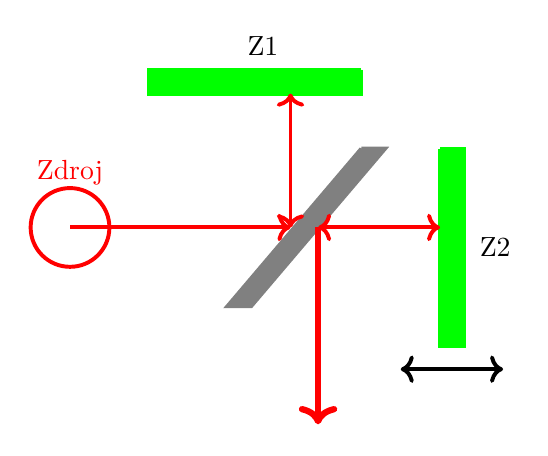
\begin{tikzpicture}
\draw[line width=0.5mm, red] (2,1) circle (0.5);
\node[red] at (2,1.7) {Zdroj};
\node at (4.45,3.3) {Z1};
\node at (7.4,0.75) {Z2};

\draw[line width=0.5mm,gray,fill=gray] (5.7,2) -- (6,2) -- (4.3,0) -- (4,0) -- (5.7,2);

\draw[line width=0.5mm,green,fill=green] (5.7,3) -- (5.7,2.7) -- (3,2.7) -- (3,3) -- (5.7,3);
\draw[line width=0.5mm,green,fill=green] (6.7,2) -- (7,2) -- (7,-0.5) -- (6.7,-0.5) -- (6.7,2);
\draw[line width=0.5mm,black,<->] (6.2,-0.8) -- (7.5,-0.8);

\draw[line width=0.5mm,red,->] (2,1) -- (4.8,1);
\draw[line width=0.5mm,red,<->] (4.8,2.7) -- (4.8,1);
\draw[line width=0.5mm,red,<->] (6.7,1) -- (5.15,1);

\draw[line width=0.8mm,red,->] (5.15,1) -- (5.15,-1.5);

\end{tikzpicture}
	\vfill
}

\subsection{Monochromátor}
\frame{
	\frametitle{}
	\vfill
	\begin{itemize}
	\item Nejčastěji se využívá \emph{difrakční mřížka}.\footnote[frame]{\href{https://www.wikiskripta.eu/w/Optick\%C3\%A1_m\%C5\%99\%C3\%AD\%C5\%BEka}{Optická mřížka}}
	\item Rozkládá dopadající světlo na vlnové délky.
	\item Skládá se z velkého počtu štěrbin nebo vrypů, na nichž dochází k difrakci.
	\item Hustota vrypů na mřížce je řádově stovky vrypů na centimetr.\footnote[frame]{\href{http://fyzika.jreichl.com/main.article/view/461-ohyb-svetla-na-mrizce}{Ohyb světla na mřížce}}
	\item Hustota vrypů a kvalita mřížky ovlivňuje rozlišení naměřeného spektra.
	\end{itemize}
	\begin{center}
	\adjincludegraphics[height=20mm]{../img/gratings.png}
	\end{center}
	\vfill
}

\subsection{Detektor}
\frame{
	\frametitle{}
	\vfill
	\begin{columns}
		\begin{column}{.85\textwidth}
			\begin{itemize}
				\item Jednokanálové detektory (Single-channel)
				\begin{itemize}
					\item Fotonásobič\footnote[frame]{\href{http://micro.magnet.fsu.edu/primer/flash/photomultiplier/}{Animace fotonásobiče}}
				\end{itemize}
				\item CCD - \textbf{C}harge \textbf{C}oupled \textbf{D}evice
				\begin{itemize}
					\item Vícekanálový detektor (Multi-channel).
					\item Disperzní spektrometry.
					\item Pracuje za laboratorní teploty nebo pro zvýšení citlivosti (snížení šumu) za teploty kapalného dusíku.
					\item Parametry CCD (velikost pixelu) určují rozlišení naměřeného spektra.
				\end{itemize}
			\end{itemize}
			\begin{figure}
				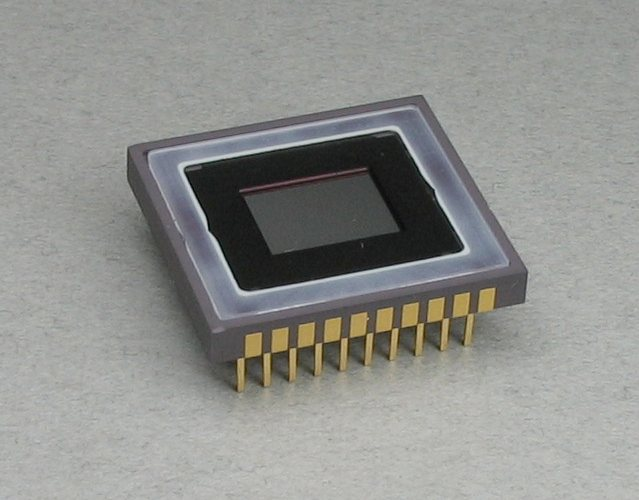
\includegraphics[height=.15\textheight]{../img/CCD.jpg}
				\caption*{CCD čip\footnote[frame]{Zdroj: \href{https://commons.wikimedia.org/wiki/File:Pmside2.jpg}{Sphl/Commons}}}
			\end{figure}
		\end{column}
		\begin{column}{.15\textwidth}
			\begin{figure}
				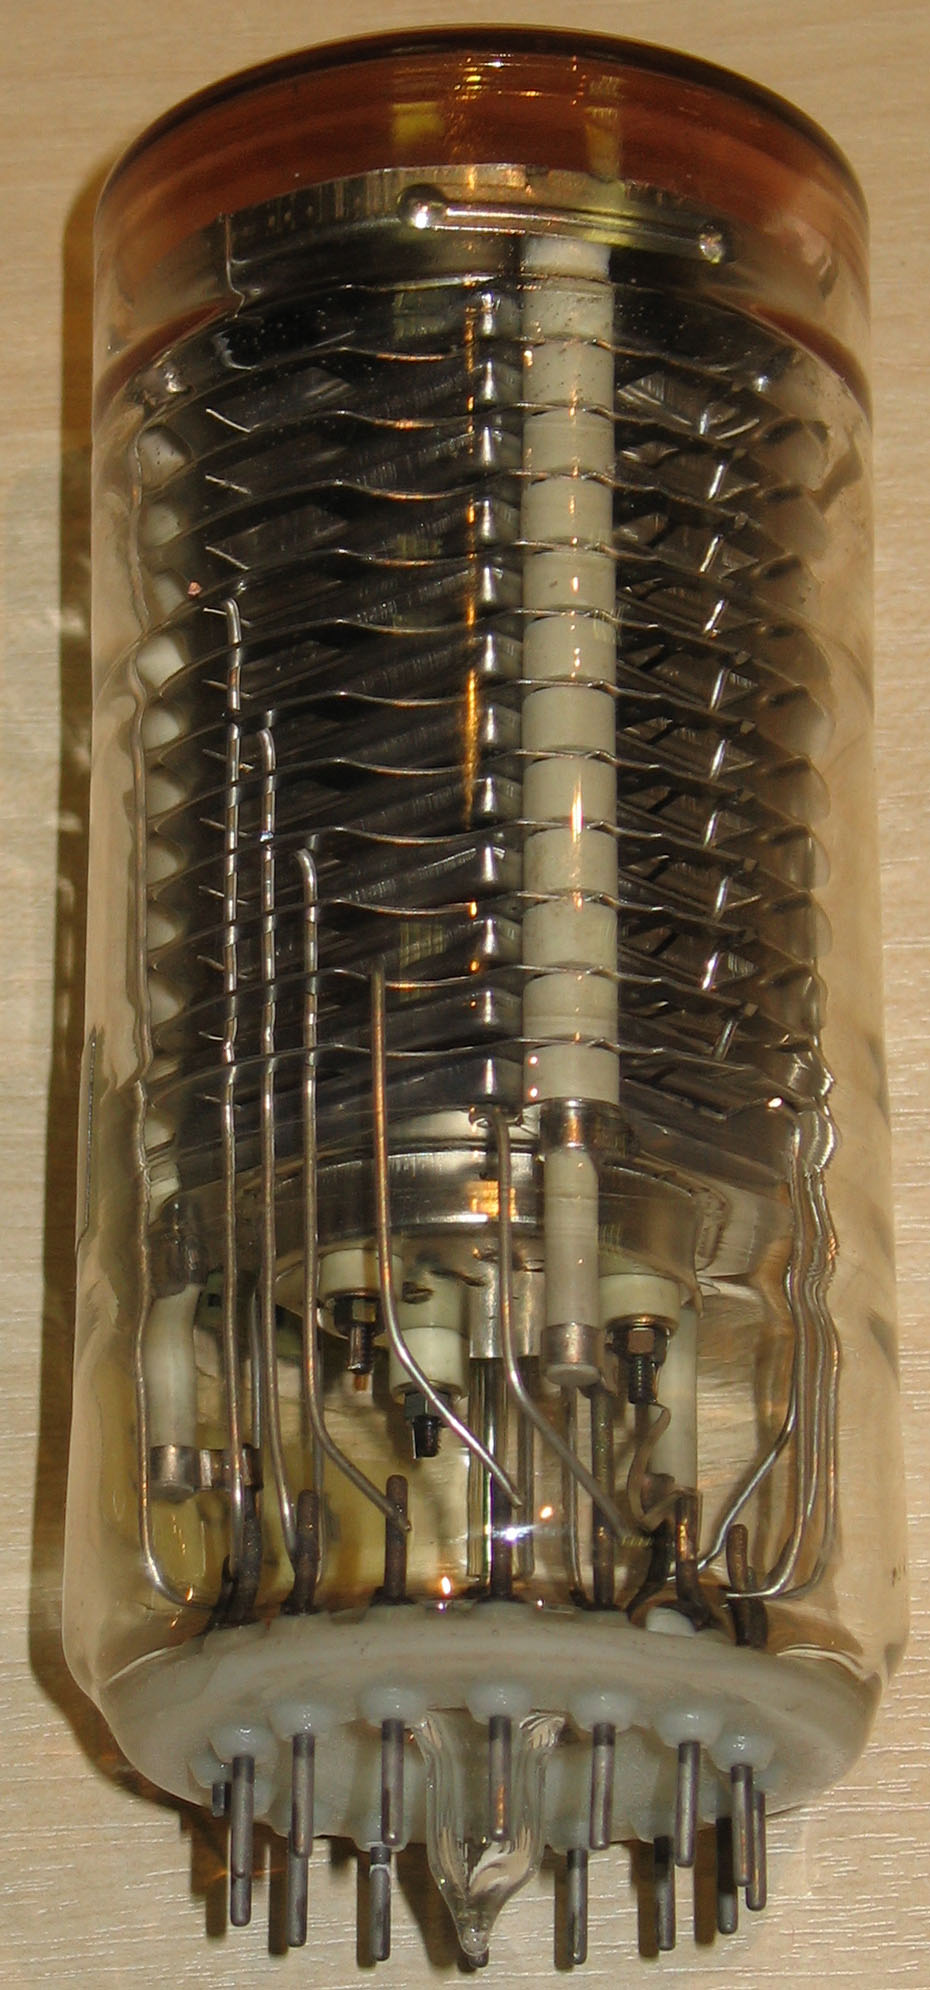
\includegraphics[width=\textwidth]{../img/Photomultipl.jpg}
				\caption*{Fotonásobič\footnote[frame]{Zdroj: \href{https://commons.wikimedia.org/wiki/File:Pmside2.jpg}{Poil/Commons}}}
			\end{figure}
		\end{column}
	\end{columns}
	\vfill
}

\subsection{Ramanova mikroskopie}
\frame{
	\frametitle{}
	\vfill
	\begin{itemize}
	\item První Ramanův mikroskop byl vyvinut v 70. letech 20. století.
	\item Umožňuje nedestruktivně měřit spektra i od větších vzorků.
	\item Umožňuje velmi přesně zaměření LASERu na požadované místo, příp. i mapování části povrchu vzorku.
	\item Velmi výhodný pro analýzu uměleckých předmětů, biologických vzorků, apod.
	\end{itemize}
	\begin{figure}
		\adjincludegraphics[height=.35\textheight]{../img/raman-microscope.jpg}
	\caption*{Ramanův mikroskop.\footnote[frame]{Zdroj: \href{https://commons.wikimedia.org/wiki/File:InVia_Raman_microscope_-_March_2008.jpg}{Matzger Lab/Commons}}}
	\end{figure}
	\vfill
}

\section{SERS --- Surface-Enhanced Raman Spectrometry}
\frame{
	\frametitle{}
	\vfill
	\begin{itemize}
	\item Tento jev byl poprvé pozorován a interpretován roku 1977.
	\item Technika, umožňující zesílení Ramanova rozptylu na molekulách adsorbovaných na kovovém substrátu.\footnote[frame]{\href{https://dx.doi.org/10.1016\%2F0009-2614\%2874\%2985388-1}{Raman Spectra of Pyridine Adsorbed at a Silver Electrode}}$^,$\footnote[frame]{\href{https://dx.doi.org/10.1021/jp970340f}{Surface-Enhanced Raman Spectra of Pyridine and Pyrazine Adsorbed on a Au(210) Single-Crystal Electrode}}
	\item Zesílení signálu může být řádově až $10^{11}$, tzn. že teoreticky lze detekovat jedinou molekulu.\footnote[frame]{\href{https://dx.doi.org/10.1021/jp0687908}{Surface Enhanced Raman Scattering Enhancement Factors}}
	\item Prakticky je však hodnota zesílení spíše 10$^3$ až 10$^6$.
	\item Jako substrát je nejvhodnější stříbro, ale využívá se také zlato a měď.\footnote[frame]{\href{https://doi.org/10.1021/acsnano.9b04224}{Present and Future of Surface-Enhanced Raman Scattering}}
	\end{itemize}
	\vfill
}

\frame{
	\frametitle{}
	\vfill
	\begin{itemize}
	\item Vznik SERS lze popsat dvěma mechanismy:
	\begin{itemize}
		\item Prvním je zesílené elektromagnetické pole vytvářené na povrchu kovu (\textit{povrchová plazmonová rezonance}). Nejvíce jsou zesilovány vibrační módy kolmé k povrchu kovu.
		\item Druhý způsob zesílení spočívá v přenosu náboje mezi povrchem a molekulou analytu. Elektronické přechody mnoha komplexů s přenosem náboje jsou ve viditelné oblasti, takže dochází k rezonančnímu zesílení. Nejsilnější SERS vykazují molekuly s nepárovými elektrony nebo pí elektrony (aromatické sloučeniny). Tento efekt byl poprvé objeven u pyridinu.
	\end{itemize}
	\item Využití SERS v praxi
	\begin{itemize}
		\item Studium povrchových vrstev analytu na kovovém substrátu.
		\item Lze také studovat koloidní a kovové filmy na dielektrických substrátech.
		\item Analýza biologických vzorků o malé koncentraci.
	\end{itemize}
	\end{itemize}
	\vfill
}

\frame{
	\frametitle{}
	\vfill
	\begin{figure}
		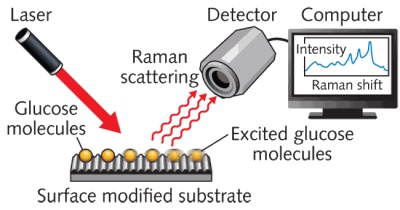
\includegraphics[height=.7\textheight]{../img/sers.jpg}
		\caption*{Ramanovo spektrum 2-merkaptoethanolu (\ce{HS-CH2-CH2-OH}): a) kapalina, b) SERS, 10 mM roztok na stříbrném substrátu.\footnote[frame]{Zdroj: \href{https://commons.wikimedia.org/wiki/File:Sers.jpg}{Paszczakowna1/Commons}}}
	\end{figure}
	\vfill
}

\section{Ramanova optická aktivita}
\frame{
	\frametitle{}
	\vfill
	\begin{columns}
		\begin{column}{.6\textwidth}
			\begin{itemize}
				\item Měřící technika, kdy zaznamenáváme rozdíl v intenzitách Ramanova rozptylu pravo- a levotočivě polarizovaného záření na chirálních molekulách.
				\item Metodu lze využít pro stanovení enantiomerické čistoty, a to i u směsí několika chirálních látek.\footnote[frame]{\href{https://journals.sagepub.com/doi/pdf/10.1177/1934578X1000500914}{Raman Optical Activity: A Powerful Technique to Investigate Essential Oil Components}}
				\item V současnosti nachází velké využití při studiu struktury biomolekul a jejich chování ve vodných roztocích.
			\end{itemize}
		\end{column}
		\begin{column}{.4\textwidth}
			\begin{figure}
				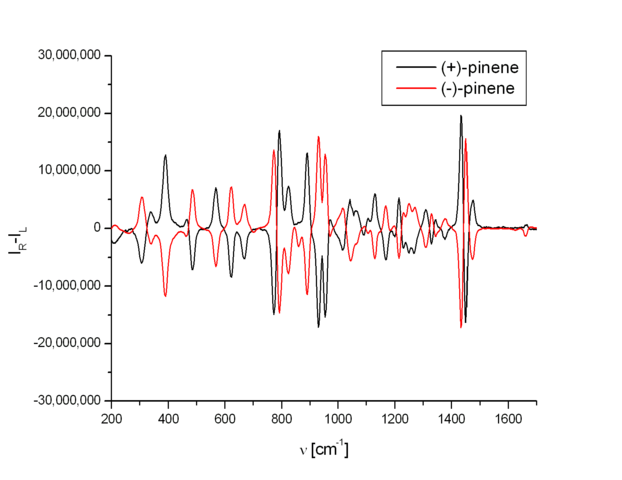
\includegraphics[width=\textwidth]{../img/ROA_pinene.png}
				\caption*{ROA spektrum (+) a (-) pinenu.\footnote[frame]{Zdroj: \href{https://commons.wikimedia.org/wiki/File:ROA_pinene.PNG}{M.Pecul/Commons}}}
			\end{figure}
		\end{column}
	\end{columns}
	\vfill
}

\section{Využití Ramanovy spektroskopie v praxi}
\frame{
	\frametitle{}
	\vfill
	\begin{itemize}
	\item \emph{Farmacie, kosmetika}
	\begin{itemize}
	\item Rozložení sloučenin v tabletě
	\item Složení a čistota práškových produktů
	\item Krystalinita
	\item Koncentrace aktivních látek
	\end{itemize}
	\item \emph{Geologie}
	\begin{itemize}
	\item Identifikace minerálů a drahokamů
	\item Fázové přechody
	\item Chování minerálů v extrémních podmínkách
	\end{itemize}
	\item \emph{Polovodičový průmysl}
	\begin{itemize}
	\item Čistota
	\item Analýza defektů
	\item Fotoluminiscenční mikroanalýza
	\item Složení slitin
	\end{itemize}
	\item \emph{Přírodní vědy}
	\begin{itemize}
	\item Analýza DNA/RNA
	\item Analýza jednotlivých buněk
	\item Struktura kostí
	\item Interakce léčiva s buňkami
	\end{itemize}
	\end{itemize}
	\vfill
}

\subsubsection{Studium struktury grafenu}
\frame{
	\frametitle{}
	\vfill
		\begin{itemize}
			\item Pomocí Ramanovy spektroskopie lze studovat kvalitu grafenu a určit počet vrstev vzorku.\footnote[frame]{\href{https://doi.org/10.1103/PhysRevLett.97.187401}{Raman Spectrum of Graphene and Graphene Layers}}
			\item Pás D (1350~cm$^{-1}$) odpovídá poruchám ve struktuře grafenu.
			\item Pás G (1583~cm$^{-1}$) odpovídá valenčním vibracím vazeb C-C, najdeme ve všech systémech s sp$^2$ uhlíky.
			\item V případě nečistot nebo výskytu náboje na povrchu grafenu, najdeme v blízkosti pásu G i méně intenzivní pás D' (1620~cm$^{-1}$).
			\item Pás G' v oblasti 2500-2800~cm$^{-1}$ se označuje jako 2D-pás, nalezneme ho u všech systému s sp$^2$ uhlíky.
			\item Zlepšení dat získaných z 2D materiálů lze dosáhnout měřením za kryogenních teplot.\footnote[frame]{\href{https://chemagazin.cz/content/id_magazines_pdf/49.pdf}{DIEING, T.; ALTMANN, P.; ENGLERT, J.; STROM, D. a BACANI, M. Kryogenní Ramanovo zobrazování šupin diselenidu wolframu. \textit{Chemagazín}. 2025, roč. XXXV, č. 1, s. 12-13.}}
		\end{itemize}
	\vfill
}

\frame{
	\frametitle{}
	\vfill
	\begin{columns}
		\begin{column}{0.5\textwidth}
			\begin{figure}
				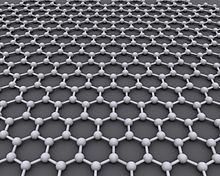
\includegraphics[width=\textwidth]{../img/Graphen.jpg}
				\caption*{Struktura grafenu.\footnote[frame]{Zdroj: \href{https://commons.wikimedia.org/wiki/File:Graphen.jpg}{AlexanderAlUS/Commons}}}
			\end{figure}
		\end{column}
		\begin{column}{0.5\textwidth}
			\begin{figure}
				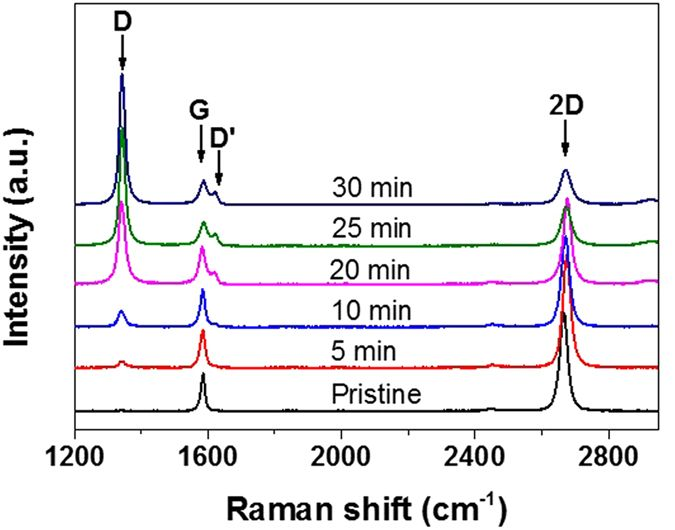
\includegraphics[width=\textwidth]{../img/Graphene_Raman_spectrum.jpg}
				\caption*{Ramanovo spektrum grafenu.\footnote[frame]{Zdroj: \href{https://commons.wikimedia.org/wiki/File:Graphene_Raman_spectrum.jpg}{Guodong Gao, Dandan Liu, Shangcheng Tang, Can Huang, Mengci He, Yu Guo, Xiudong Sun \& Bo Gao/Commons}}}
			\end{figure}
		\end{column}
	\end{columns}
	\vfill
}

\subsection{Analýza uměleckých předmětů}
\frame{
	\frametitle{}
	\vfill
	\begin{itemize}
	\item Spektroskopická analýza uměleckých předmětů je velice důležitá pro konzervátory, historiky umění i sběratele.\footnote[frame]{\url{http://www.ndt.net/article/wcndt00/papers/idn163/idn163.htm}}$^,$\footnote[frame]{\href{http://dx.doi.org/10.1002/1097-4555(200006)31:6<509::AID-JRS566>3.0.CO;2-0}{Raman spectroscopic database of azo pigments and application to modern art studies}}
	\item Ramanova spektroskopie a mikroskopie se využívá pro:\footnote[frame]{\href{http://dx.doi.org/10.1016/S1386-1425(00)00495-9}{Library of FT-Raman spectra of pigments, minerals, pigment media and varnishes, and supplement to existing library of Raman spectra of pigments with visible excitation}}
	\begin{itemize}
	\item Identifikaci anorganických pigmentů
	\item Identifikaci organických pigmentů
	\item Identifikaci pojiv a laků
	\end{itemize}
	\item Větší předměty, např. nástěnné malby lze analyzovat s využitím optických vláken, aniž by hrozilo jejich poškození.\footnote[frame]{\href{http://www.ncbi.nlm.nih.gov/pmc/articles/PMC1802725/}{Non-destructive analysis of museum objects by fibre-optic Raman spectroscopy}}
	\end{itemize}
	\vfill
}

\subsection{Analýza biologických vzorků}
\frame{
	\frametitle{}
	\vfill
	\begin{itemize}
		\item Ramanovu spektroskopii lze využít jako neinvazivní, a přitom rychlou a přesnou metodu detekce karcinomu tlustého střeva.\footnote[frame]{\href{https://doi.org/10.1039/D3AN00103B}{\textit{In vivo} Raman spectroscopy in the diagnostics of colon cancer}}
		\item Vzorky lze získat během diagnostické kolonoskopie.
		\item Analýza spekter byla provedena s využitím metod strojového učení.
		\item Oproti běžným diagnostickým metodám lze získat i další informace o složení tkání.
	\end{itemize}
	\begin{center}
		\begin{tabular}{|l|l|l|}
			\hline
			\textbf{Pás [cm$^{-1}$]} & \textbf{Vibrační mód} & \textbf{Přiřazení} \\\hline
			935 & $\nu$ (CC) & proteiny, $\alpha$-helix, Pro, Val \\\hline
			1005 & $\delta$ (CC) dýchání kruhu & Phe \\\hline
			1050 & $\nu$ (CN), $\nu$ (CO) & Pro \\\hline
			1077 & $\nu$ (CC), $\nu$ (CO) & Glukóza, triglyceridy, lipidy \\\hline
			1126 & $\nu$ (CN), $\nu$ (CC) & Proteiny, lipidy, fosfolipidy \\\hline
			1750 & $\nu$ (C=O) & Lipidy, fosfolipidy \\\hline
		\end{tabular}
	\end{center}
	\vfill
}

\frame{
	\frametitle{}
	\vfill
	\begin{itemize}
	\item S výhodou lze využít fluorescenční mikroskopy s Ramanovým spektrometrem.
	\item Na obrázku jsou buňky primátů obarvené fluorescenčním barvivem DAPI a příslušné Ramanovo spektrum.\footnote[frame]{\href{https://chemagazin.cz/archiv-casopisu/chemagazin-5-2019}{CHEMAGAZIN, 2019, 5, 22-23}}
	\item Pro excitaci byl využit laser o vlnové délce 532~nm. Byl získán obrázek plochy $50\times 40\ \mu $m.
	\item Jádra buněk jsou znázorněna modře, jadérka zeleně a endoplazmatická retikula červeně.
	\end{itemize}
	\begin{figure}
		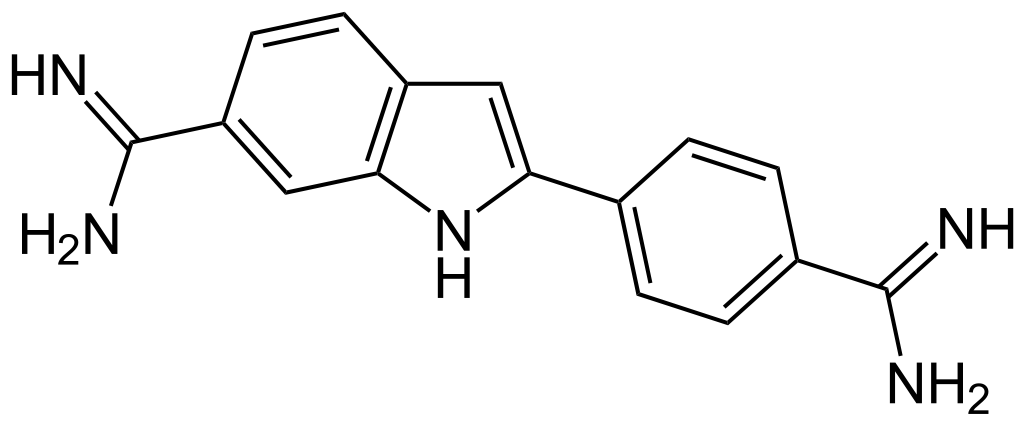
\includegraphics[width=.6\textwidth]{../img/DAPI.png}
	\end{figure}
	\vfill
}

\frame{
	\frametitle{}
	\vfill
	\begin{figure}
		\adjincludegraphics[width=\textwidth]{../img/RA-primati-BIO.png}
	\end{figure}
	\vfill
}

\subsection{Analýza mikroplastů}
\frame{
	\frametitle{}
	\vfill
	\begin{itemize}
		\item Ramanova mikroskopie je důležitou metodou pro analýzu mikroplastů v životním prostředí a organismech.
	\end{itemize}
	\begin{figure}
		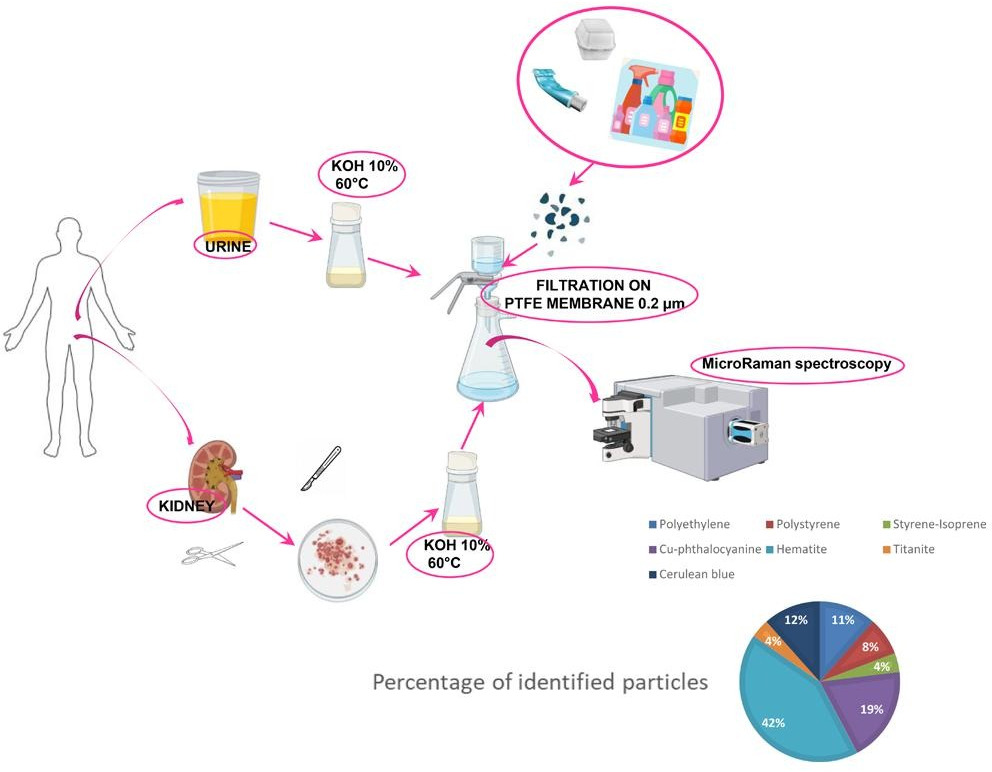
\includegraphics[height=.5\textheight]{../img/RA-microplastics.jpg}
		\caption*{Schéma izolace a analýzy mikroplastů.\footnote[frame]{\href{https://doi.org/10.1016/j.envint.2024.108444}{MicroRaman spectroscopy detects the presence of microplastics in human urine and kidney tissue}}}
	\end{figure}
	\vfill
}

\section{Spektrometry na ústavu chemie}
\frame{
	\frametitle{}
	\vfill
	\begin{itemize}
	\item IR spektrometry
	\begin{itemize}
	\item MIR spektrometr Bruker IFS 28
	\item FT-IR ( NIR+MIR) spektrometr Bruker Equinox IFS 55/S s Ramanovým nástavcem FRA 106/S
	\item FT-IR ( NIR+MIR) spektrometr Bruker Tensor 27 s možností měření TG/IR
	\item ATR Bruker Alpha Platinum
	\end{itemize}
	\item RA spektrometry
	\begin{itemize}
	\item FT-IR ( NIR+MIR) spektrometr Bruker Equinox IFS 55/S s Ramanovým nástavcem FRA 106/S
	\item Mikro-ramanovský spektrometr Horiba –  Labram HR Evolution
	\end{itemize}
	\end{itemize}
	\vfill
}

\subsection{MIR spektrometr Bruker IFS 28}
\frame{
	\frametitle{}
	\vfill
	\begin{center}
	\adjincludegraphics[width=\textwidth]{../img/ifs28.jpg}
	\end{center}
	\vfill
}

\subsection{Bruker Equinox IFS 55/S s Ramanovým nástavcem FRA 106/S}
\frame{
	\frametitle{}
	\vfill
	\begin{center}
	\adjincludegraphics[width=\textwidth]{../img/equinox.jpg}
	\end{center}
	\vfill
}

\subsection{Bruker Tensor 27}
\frame{
	\frametitle{}
	\vfill
\begin{figure}
 \centering
   \begin{tikzpicture}[overlay]
     \node at (0,0) {\adjincludegraphics[scale=0.35]{../img/tg-irFoto.jpg}};
     \node at (-3,2.1) {\adjincludegraphics[width=5cm]{../img/tensor-ATR.png}};
  \end{tikzpicture}
\end{figure}
	\vfill
}

\subsection{Bruker Alpha Platinum}
\frame{
	\frametitle{}
	\vfill
	\adjincludegraphics[scale=0.35]{../img/alpha.jpg}
	\vfill
}

\subsection{Mikro-ramanovský spektrometr Horiba –  Labram HR Evolution - UGV}
\frame{
	\frametitle{}
	\vfill
	\begin{itemize}
	\item \url{https://ugv.sci.muni.cz/veda-a-vyzkum/sluzby/pracoviste-ramanovy-spektroskopie}
	\end{itemize}
	\adjincludegraphics[height=5cm]{../img/raman-geo.jpg}
	\vfill
}

\end{document}
